\documentclass{article}
\usepackage{amsmath}
\usepackage{graphicx}
\begin{document}
\author{Ana Bhattacharjee}
\title{Parallel and Perpendicular Lines: Question 16}
\date{\today}
\maketitle{}

\begin{center}
The picture of triangle PQR is shown below.
\par
\begin{figure}[!htbp]
  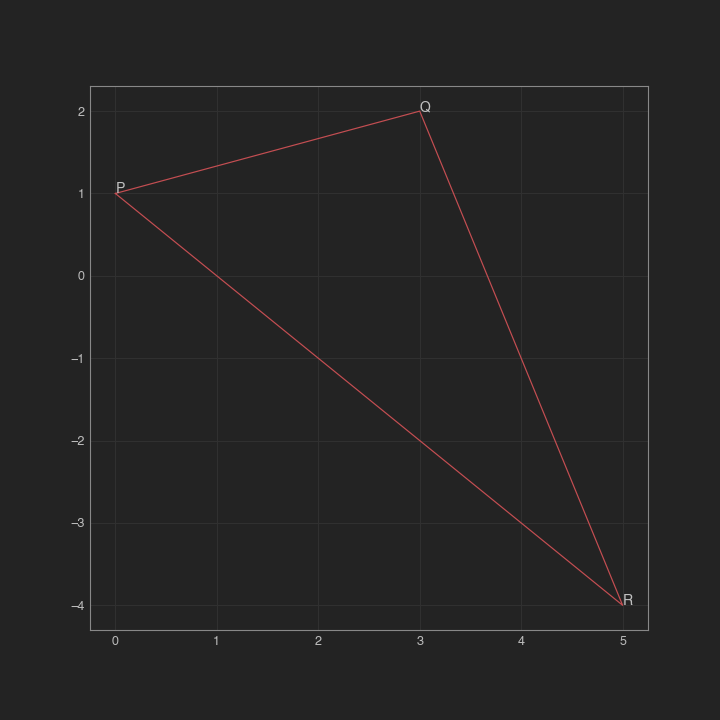
\includegraphics[width=1.0\columnwidth]{polygon}
  \caption{Triangle PQR}
\end{figure}
\par
From the triangle above, I will calculate the slopes of PQ and QR to see whether or not the triangle is a right triangle.
\begin{align}
  \text{slope}_{PQ} = \frac{2 - 1}{3 - 0} = \frac{1}{3} \\
  \text{slope}_{QR} = \frac{-4 - 2}{5 - 3} = \frac{-6}{2} = -3 \\
  \frac{1}{3} * -3 = -1
\end{align}
Since the slopes, when multiplied together, retrieve a product of -1, the triangle PQR is a right triangle. 
\end{center}

\end{document}
